\subsection{Arduino UNO R3}

Esta tarjeta se encarga de recibir y almacenar el orden de cada señal entregada ~\cite{buitrago}. 

Es el microcontrolador principal que controla todas las funciones básicas del sistema, como leer datos de los sensores (nivel de llenado, detección de movimiento) y activar los actuadores (abrir/cerrar la tapa del cubo). También es el que recibe las señales de los sensores y ejecuta las acciones correspondientes, como encender un buzzer o enviar alertas.


\begin{figure}[htb]
	\centering
	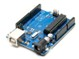
\includegraphics[scale  = 0.50]{Imagenes/uno3.jpg}
	\caption{ARDUINO UNO R3 }{Fuente: Adaptado de~\cite{mecafenix}}

\end{figure}

\subsection{IDE Arduino}

El entorno de programaciónde la  placa  de  Arduino  se denomina Integrated  Development  Environment (IDE)el cual  permite  llevar  a  cabo  la  escritura  de  las  sentencias para el funcionamiento de los elementos físicos de la placa de Arduino. Este   software   tiene   por   si   solo   un   conjunto   de herramientas que permite,  editar  el  código,  compilar  y depurar todo a través de una interfaz gráfica, así mismo, nos    da    la    oportunidad    de    interactuar    con    el microcontrolador almacenando los programas  realizados en  su  memoria  interna  para  poner  en  marcha  todo  el hardware. El lenguaje que utiliza el IDE de Arduino está basado en C/C++ de una manera más simplificada, ofreciendo la oportunidad de cargar librerías que sean necesarias para el buen funcionamiento de nuestros proyectos ~\cite{perez}.

\begin{figure}[htb]
	\centering
	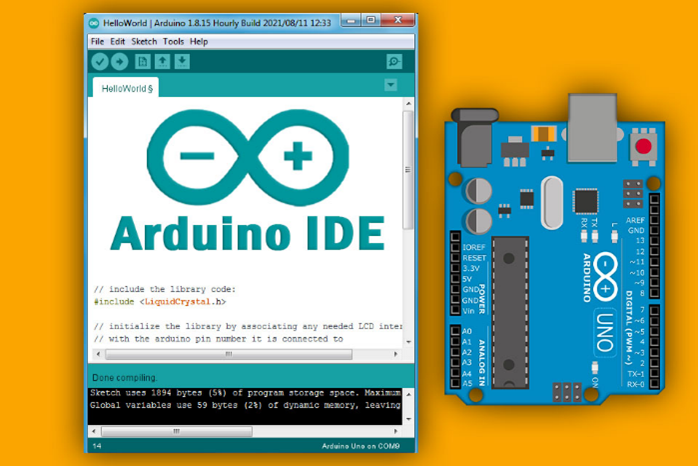
\includegraphics[scale  = 0.80]{Imagenes/ide.png}
	\caption{IDE Arduino}{Fuente: Adaptado de~\cite{perez}}

\end{figure}

\subsection{Micropython}

MicroPython es una reimplementación del lenguaje de programación Python que apunta a microcontroladores y sistemas integrados.

Los microcontroladores son computadoras compactadas en un solo chip muy pequeño. Los sistemas integrados son computadoras que funcionan dentro de un sistema mecánico o eléctrico más grande~\cite{tollervey}.

Los sistemas integrados a menudo utilizan microcontroladores.

\begin{figure}[H]
	\centering
	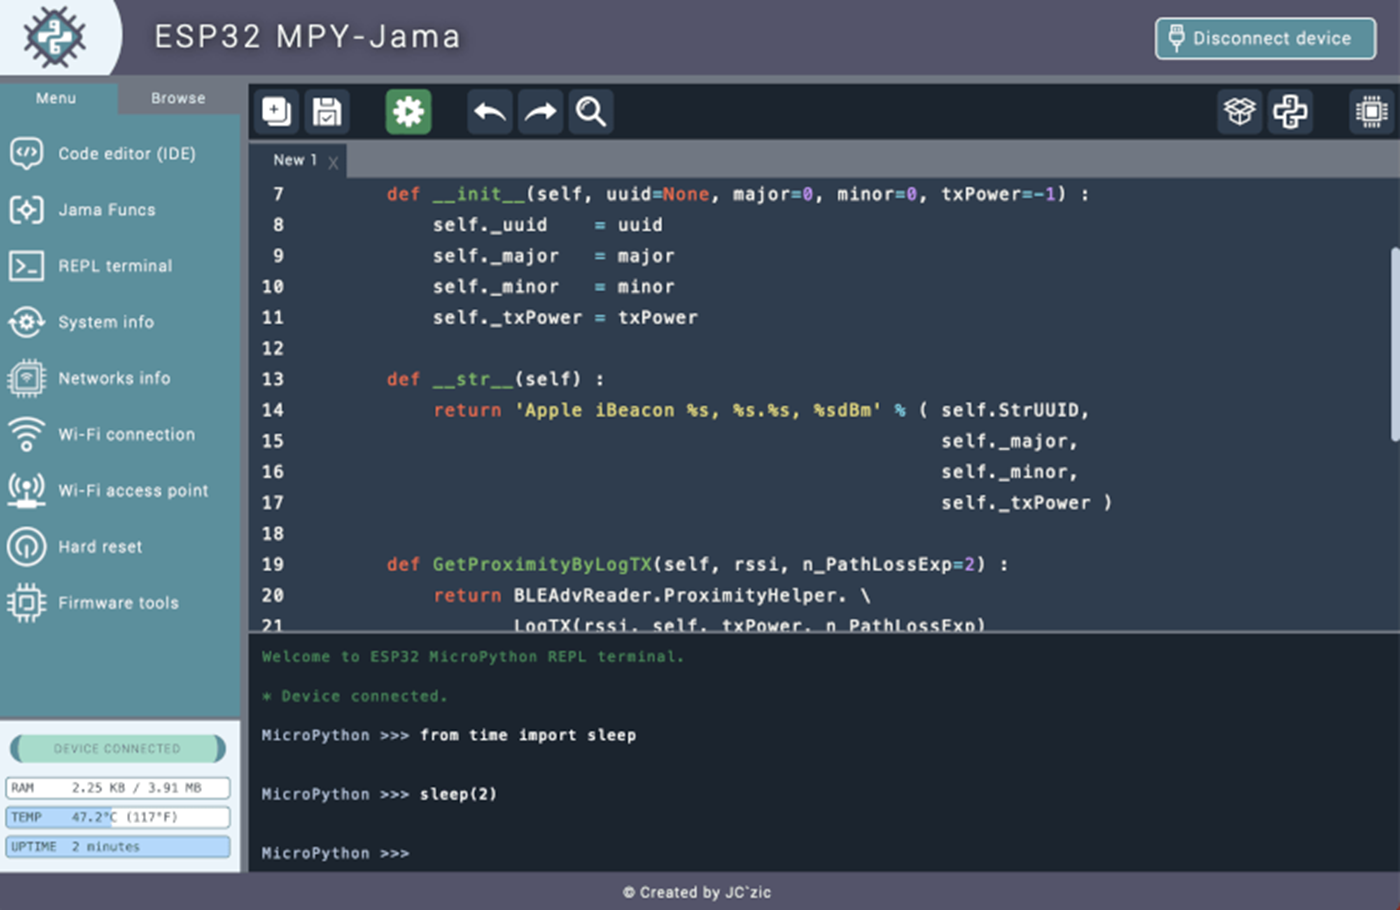
\includegraphics[scale  = 0.60]{Imagenes/mycro.png}
	\caption{Interfaz de MicroPython}{Fuente: Adaptado de~\cite{mpy}}
\end{figure}


\subsection{CNN}

Una red neuronal convolucional es un tipo de red neuronal artificial donde las neuronas artificiales, corresponden a campos receptivos de una manera muy similar a las neuronas en la corteza visual primaria (V1) de un cerebro biológico. Este tipo de red es una variación de un perceptron multicapa, sin embargo, debido a que su aplicación es realizada en matrices bidimensionales, son muy efectivas para tareas de visión artificial, como en la clasificación y segmentación de imágenes, entre otras aplicaciones~\cite{red_neuronal}.

\begin{figure}[htb]
	\centering
	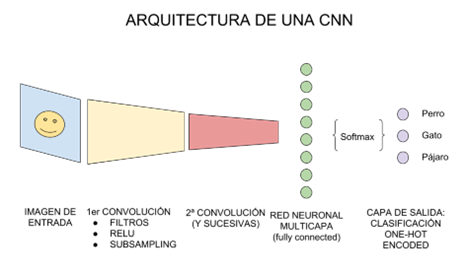
\includegraphics[scale  = 0.80]{Imagenes/cnn.png}
	\caption{Arquitectura de una red CNN}{Fuente: Adaptado de~\cite{red_neuronal}}

\end{figure}

\subsection{Visión Artificial}

Es una disciplina científica que incluye métodos para adquirir, procesar, analizar y comprender las imágenes del mundo real con el fin de producir información numérica o simbólica para que puedan ser tratados por un ordenador. Tal y como los seres humanos usamos nuestros ojos y cerebros para comprender el mundo que nos rodea, la visión informática trata de producir el mismo efecto para que los ordenadores puedan percibir y comprender una imagen o secuencia de imágenes y actuar según convenga en una determinada situación. Esta comprensión se consigue gracias a distintos campos como la geometría, la estadística, la física y otras disciplinas. La adquisición de los datos se consigue por varios medios como secuencias de imágenes, vistas desde varias cámaras de video o datos multidimensionales desde un escáner médico~\cite{vision_artificial}.

\subsection{Open CV}

\textbf{OpenCV} es una biblioteca libre de visión artificial originalmente desarrollada por Intel. OpenCV significa Open Computer Vision (Visión Artificial Abierta). OpenCV ofrece soporte para varios sistemas operativos y varias arquitecturas de hardware, pero también ofrece el código fuente para que cualquier desarrollador lo compile en cualquier sistemas operativo y arquitectura particular~\cite{opencv}. 

OpenCV y ESP32 se pueden utilizar juntos para crear sistemas de visión integrados, en los que se pueden ejecutar tareas de visión por computadora simples en un microcontrolador ESP32.

\begin{figure}[htb]
	\centering
	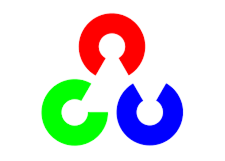
\includegraphics[scale  = 0.80]{Imagenes/opencv.png}
	\caption{Logo de OpenCV}{Fuente: Adaptado de~\cite{opencv}}

\end{figure}

\subsubsection{Numpy}

NumPy es una biblioteca para el lenguaje de programación Python, que agrega soporte para matrices y arreglos multidimensionales grandes, junto con una gran colección de funciones matemáticas de alto nivel para operar en estos arreglos~\cite{numpy}.

\begin{figure}[htb]
	\centering
	
\includegraphics[scale  = 0.80]{Imagenes/numpy.png}
	\caption{Logo de Numpy}{Fuente: Adaptado de~\cite{numpy}}
\end{figure}

\subsection{XIAO ESP32 CAM}
El ESP32-CAM es un módulo de cámara muy pequeño y económico que cuenta con el chip ESP32-S. Además de la cámara OV2640 y varios GPIO para conectar periféricos, también cuenta con una ranura para tarjeta microSD que puede ser útil para almacenar imágenes tomadas con la cámara o para almacenar archivos para servir a los clientes 

\begin{figure}[htb]
	\centering
	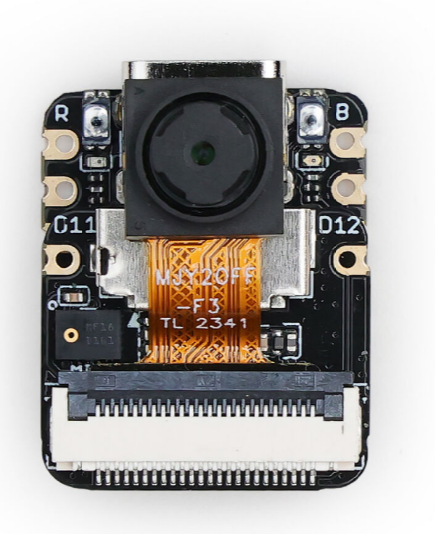
\includegraphics[scale  = 0.70]{Imagenes/xiao.png}
	\caption{XIAO ESP32 CAM}{Fuente: Adaptado de~\cite{foto_xiao}}
\end{figure}

A continuación, se presenta el DataSheet encontrado.

\begin{table}[H]
    \centering
    \begin{tabularx}{\textwidth}{|l|X|} % Usar X para columnas que se expanden
        \hline
        \textbf{Ítem} & \textbf{Descripción} \\ 
        \hline
        \textbf{Procesador} & ESP32-S3R8, Xtensa LX7 de doble núcleo, 32 bits, hasta 240 MHz \\ 
        \hline
        \textbf{Inalámbrico} & Subsistema Wi-Fi completo de 2.4GHz, BLE: Bluetooth 5.0, Bluetooth mesh \\ 
        \hline
        \textbf{Sensores Integrados} & Sensor de cámara OV2640 (1600*1200), Micrófono digital \\ 
        \hline
        \textbf{Memoria} & 8M PSRAM y 8MB Flash en chip, Ranura para tarjeta SD (hasta 32GB FAT) \\ 
        \hline
        \textbf{Interfaz} & 1x UART, 1x IIC, 1x IIS, 1x SPI, 11x GPIOs (PWM), 9x ADC, 1x LED de usuario, 1x LED de carga \\ 
        & 1x conector B2B (2 GPIOs adicionales), 1x botón de reinicio, 1x botón de arranque \\ 
        \hline
        \textbf{Dimensiones} & 21 x 17.8 x 15 mm (con placa de expansión) \\ 
        \hline
        \textbf{Alimentación} & Voltaje de entrada (Type-C): 5V, Voltaje de entrada (BAT): 4.2V \\ 
        & Voltaje de operación (Type-C): 5V@38.3mA, Voltaje de operación (BAT): 3.8V@43.2mA (con expansión) \\ 
        \hline
        \textbf{Modelo de Bajo Consumo} & Sueño de módem: ~44mA, Sueño ligero: ~5mA, Sueño profundo: ~3mA \\ 
        \hline
        \textbf{Consumo de Potencia (Wi-Fi)} & Modelo activo: ~110 mA (con expansión) \\ 
        \hline
        \textbf{Consumo de Potencia (BLE)} & Modelo activo: ~102 mA (con expansión) \\ 
        \hline
        \textbf{Temperatura de Funcionamiento} & -40°C ~ 65°C \\ 
        \hline
    \end{tabularx}
    \caption{DataSheet de la XIAO ESP32 CAM}{Fuente: ~\cite{xiaotabla}}
\end{table}

\subsection{Sensor ultrasónico (HC-SR04)}

Este sensor mide la distancia entre el sensor y el nivel de basura dentro del cubo. Con esta información, se puede calcular el porcentaje de llenado. Funciona enviando pulsos ultrasónicos y midiendo el tiempo que tarda en regresar el eco, lo que indica la distancia al objeto más cercano (en este caso, la basura).

\begin{figure}[htb]
	\centering
	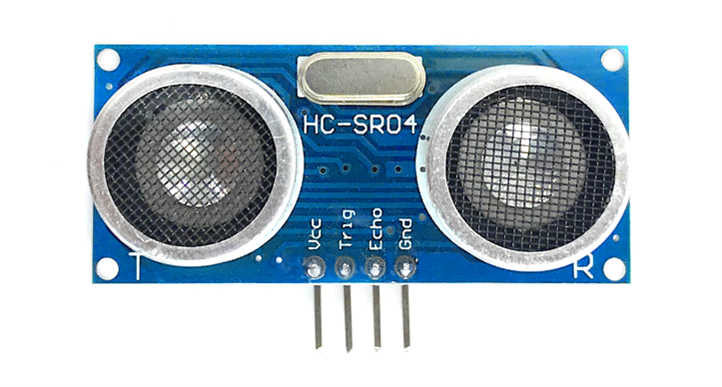
\includegraphics[scale  = 0.50]{Imagenes/ultra.png}
	\caption{Sensor ultrasónico HC-SR04}{Fuente: Adaptado de~\cite{ultrasonc}}

\end{figure}

\begin{table}[H]
    \centering
    \begin{tabularx}{\textwidth}{|l|X|} % Usar X para columnas que se expanden
        \hline
        \textbf{Especificación} & \textbf{Descripción} \\ 
        \hline
        \textbf{Voltaje de funcionamiento} & DC 5V \\ 
        \hline
        \textbf{Corriente de funcionamiento} & 15mA \\ 
        \hline
        \textbf{Frecuencia de funcionamiento} & 40kHz \\ 
        \hline
        \textbf{Alcance máximo} & 4 m \\ 
        \hline
        \textbf{Alcance mínimo} & 2 cm \\ 
        \hline
        \textbf{Precisión de medición} & 3 mm \\ 
        \hline
        \textbf{Ángulo de medición} & 15 grados \\ 
        \hline
        \textbf{Señal de entrada del disparador} & Pulso TTL de 10 µs \\ 
        \hline
        \textbf{Dimensiones} & 45 x 20 x 15 mm \\ 
        \hline
    \end{tabularx}
    \caption{Especificaciones del HC-SR04}{Fuente: Adaptado de~\cite{ultrasonc}}
    \label{tab:especificaciones_hc_sr04}
\end{table}

\subsection{Cables jumper, resistencias, protoboard}

Estos componentes se utilizan para conectar todos los sensores, microcontroladores y actuadores de manera temporal o durante la fase de pruebas. Los cables jumper permiten hacer conexiones rápidas entre pines, y la protoboard facilita las conexiones sin necesidad de soldar.

\begin{figure}[htb]
	\centering
	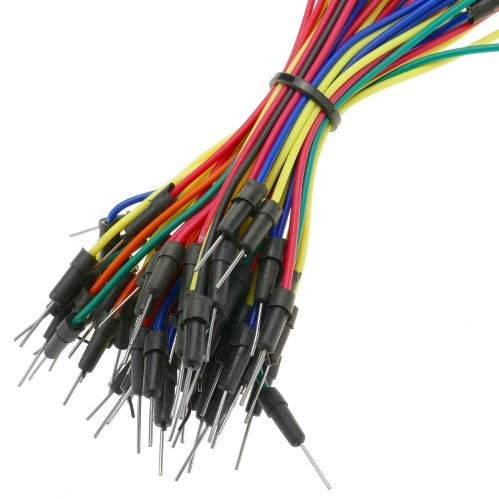
\includegraphics[scale  = 0.50]{Imagenes/jumper.jpg}
	\caption{Jumpers}{Fuente: Propia}
\end{figure}

\begin{figure}[htb]
	\centering
	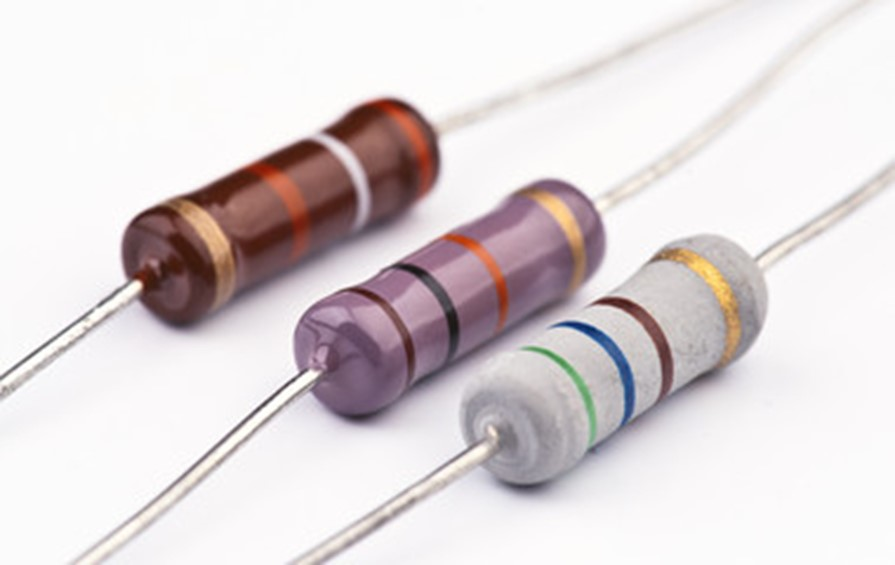
\includegraphics[scale  = 0.50]{Imagenes/resistores.jpg}
	\caption{Resistores}{Fuente: Propia}
\end{figure}

\begin{figure}[htb]
	\centering
	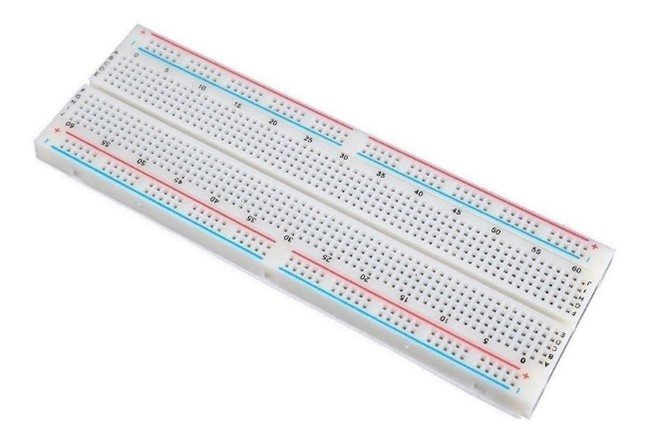
\includegraphics[scale  = 0.50]{Imagenes/bread.jpg}
	\caption{ProtoBoard}{Fuente: Propia}
\end{figure}

\subsection{Servomotor (SG90)}
El SG90 es un servo miniatura de gran calidad y diminutas dimensiones, además es bastante económico. Funciona con la mayoría de las tarjetas electrónicas de control con microcontroladores y además con la mayoría de los sistemas de radio control comerciales. Funciona especialmente bien en aeronaves dadas sus características de torque, tamaño y peso.

El servo SG90 tiene un conector universal tipo “S” que encaja perfectamente en la mayoría de los receptores de radio control incluyendo los Futaba, JR, GWS, Cirrus, Hitec y otros. Los cables en el conector están distribuidos de la siguiente forma: Rojo = Alimentación (+), Cafe = Alimentación (-) o tierra, Naranjo = Señal PWM.

Este tipo de servo es ideal para las primeras experiencias de aprendizaje y prácticas con servos, ya que sus requerimientos de energía son bastante bajos y se permite alimentarlo con la misma fuente de alimentación que el circuito de control. Por ejemplo, si se conecta a una tarjeta arduino, se puede alimentar durante las pruebas desde el puerto USB de la PC sin mayor problema~\cite{servo_motor}.

\begin{figure}[H]
	\centering
	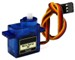
\includegraphics[scale  = 0.50]{Imagenes/micro.jpg}
	\caption{Mini Sevo motor}{Fuente: Adaptado de~\cite{servo_motor}}
\end{figure}

A continuación, se muestra el DataSheet encontrado:

\begin{table}[H]
    \centering
    \begin{tabularx}{\textwidth}{|l|X|} % Usar X para columnas que se expanden
        \hline
        \textbf{Especificación} & \textbf{Descripción} \\ 
        \hline
        \textbf{Dimensiones} & 22mm x 11,5mm x 27mm \\ 
        \hline
        \textbf{Peso} & 9 gramos \\ 
        \hline
        \textbf{Peso con cable y conector} & 10.6 gramos \\ 
        \hline
        \textbf{Torque a 4.8 volts} & 1.2 kg/cm \\ 
        \hline
        \textbf{Voltaje de operación} & 4.0 a 7.2 volts \\ 
        \hline
        \textbf{Velocidad de giro a 4.8 volts} & 120 ms / 60 º \\ 
        \hline
        \textbf{Conector} & Universal para la mayoría de los receptores de radio control \\ 
        \hline
        \textbf{Compatibilidad} & Compatible con tarjetas como Arduino y microcontroladores que funcionan a 5 volts. \\ 
        \hline
    \end{tabularx}
    \caption{Especificaciones del SG90}{Fuente: Adaptado de~\cite{servo_motor}}
    \label{tab:especificaciones_sg90}
\end{table}